In this section, the method chosen to perform simulations for both the top and stop decays are shown. In addition, the preparation of data is explained in order to jusitfy the usage of ML and their results.\\
%-------------------------------------------------------------------------%
\section{Background and Signal of interest}
As discussed earlier, MadGraph5 is the chosen software to perform particle collider simulations, in which one million events were produced. At the generator level, in order to meet the pre-selection criteria (which will be discussed in the section following), we limit the missing transverse energy $\cancel{\it{E}}_{T}$ to a minimum of 200 GeV as the signatures significantly differ between tops and stops, affecting the results upon building the classifiers. Since the decay process involves both leptonic and hadronic particles as seen in Figure \ref{fig:decayDiag}, the following were defined in order to make the simulation complete. \\

\begin{lstlisting}[mathescape = true]
        define leptonic = l+ l- ta+ ta- vl vl$\sim$
        define hadronic = u c d s u$\sim$ c$\sim$ d$\sim$ s$\sim$ b b$\sim$
\end{lstlisting}

For the background process defined by Equation (\ref{eq:background}), the command to generate the events is given by
\begin{lstlisting}[mathescape = true]
            generate p p > t t$\sim$ , 
            (t > W+ b , W+ > leptonic leptonic), 
            (t$\sim$ > W- b$\sim$, W- > hadronic hadronic)
        
            add process p p > t1 t1$\sim$ ,
            (t > W+ b , W+ > hadronic hadronic), 
            (t$\sim$ > W- b$\sim$, W- > leptonic leptonic)
\end{lstlisting}
where a diagram from one of its generated events can be seen in Figure \ref{fig:bkrdFeyn}. \\

\begin{figure}[htbp]
    \centering
    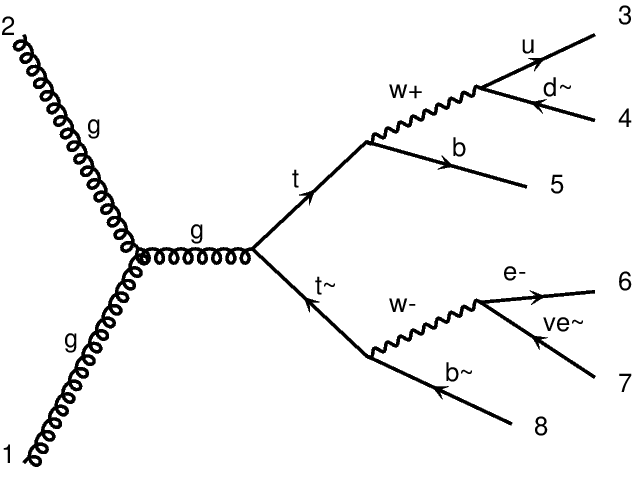
\includegraphics[width=8cm, height= 6.5cm]{top_MG5.png}
    \caption{Feynman diagram of the leading order background process $pp \rightarrow t \Bar{t} \rightarrow b\Bar{b}l^{+}jj\cancel{\it{E}}_{T} $}
    \label{fig:bkrdFeyn}
\end{figure}


Similarly, the process for signal production follows that of Equation (\ref{eq:signal}), in which the command for generating the events is given by
\begin{lstlisting}[mathescape = true]
        generate p p > t1 t1$\sim$ ,
        (t1 > t n1, (t > W+ b , W+ > leptonic leptonic)),
        (t1~ > t$\sim$ n1, (t$\sim$ > W- b$\sim$, W- > hadronic hadronic))
        
        add process p p > t1 t1$\sim$ , 
        (t1 > t n1, (t > W+ b , W+ > hadronic hadronic)), 
        (t1$\sim$ > t$\sim$ n1, (t$\sim$ > W- b$\sim$, W- > leptonic leptonic))
\end{lstlisting}
with an accompanying example diagram given in Figure \ref{fig:sigFeyn}. \\


\begin{figure}[htbp]
    \centering
    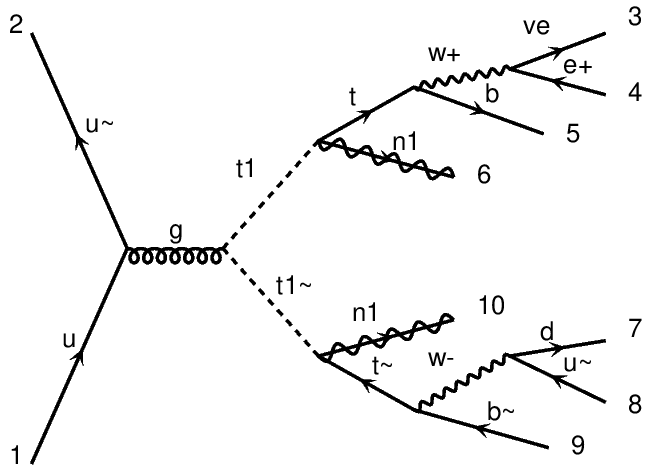
\includegraphics[width=8cm, height= 6.5cm]{stop_MG5.png}
    \caption{Feynman diagram of the leading order signal process $ pp \rightarrow \Tilde{t}\Tilde{t^*} \rightarrow t \Bar{t} \chi^0_1\chi^0_1 \rightarrow b\Bar{b}l^{+}jj\cancel{\it{E}}_{T} $ where the final states are identical to that of the background in Figure \ref{fig:bkrdFeyn}. }
    \label{fig:sigFeyn}
\end{figure}



%-------------------------------------------------------------------------%
\section{Cut flow analysis}
Methods such as, cut-flow analyses \cite{kraml2016scalar, aad2014search} and random grid searches (RGS) \cite{bhat2018optimizing} have been applied in order to optimize signal selection. Seen in Figure \ref{fig:cut} is a simple flow diagram depicting a cut-flow analysis. Each node requires a certain parameter, whether it is based on a value for a particular variable or a function of a mix of variables within the parameter space. For example, for some measurement $x$ and $y$ we could separate the signal and background, which could be further split with a 'new' parameter based on the variables $x$ and $y$ - i.e. $f(x,y)$. The final output is considered when the signal-to-background (SBR) or signal-to-noise (SNR) ratio is maximized.
This works well especially when the appropriate parameters are applied. However, there already exists at least two shortcomings with this method - the physics assumed at each node must be correct and that any selections that do not satisfy these criteria are quickly dismissed. This is the foundation for our pre-selection. \\

\begin{figure}[htbp]
    \centering
    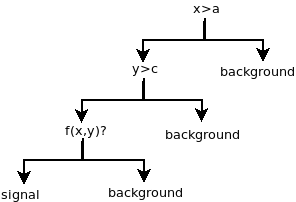
\includegraphics[width=8cm, height= 6cm]{Diagram2.png}
    \caption{Diagram depicting the flow of a cut-based analysis with arbitrary cuts $x$, $y$ and $f(x,y)$, where the final outcome has maximized SNR.}
    \label{fig:cut}
\end{figure}

Through various CMS papaers (INSERT REFERENCES HERE), our pre-selection criteria reduces down to INSERT PRE-SELECTION CRITERIA HERE MAYBE WTH A TABLE!!\\
INCLUDE PLOTS FROM MADANALYSIS

\begin{figure}[htbp]
    \centering
    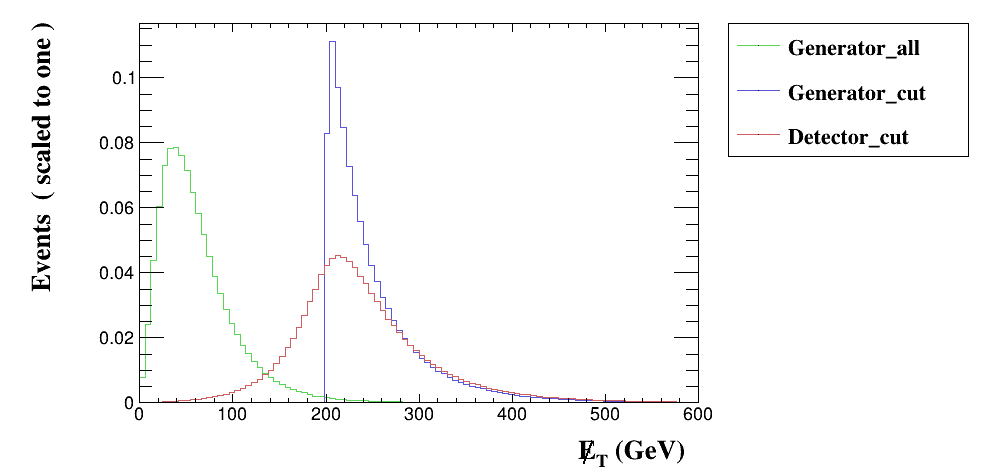
\includegraphics[width=0.75\linewidth]{top-MET.png}
    \caption{A histogram to depict the variation in generator-level and detector-level simulation.}
    \label{fig:topMET}
\end{figure}


\begin{table}[htbp]
    \centering
    \begin{tabular}{c|c|c|c|c} 
    \toprule
    Data & Initial & $\cancel{\it{E}}_{T}>250$GeV & $1l^\pm$ & $\min(1b)$ \\
    \midrule
    \rowcolor{gray!6} Benchmark1 & 776800 & 559371 & 179472 & 101488 \\
    Benchmark2 & 758458 & 611119 & 187179 & 101488 \\
    \rowcolor{gray!6} Benchmark3 & 758498 & 643458 & 191944 & 101488 \\
    Benchmark4 & 818636 & 515694 & 172171 &101488  \\
    \rowcolor{gray!6} Background & $10^6$ & 357273 & 123933 & 101488 \\
    \bottomrule
    \end{tabular}
    \caption{The number of events remaining at each step of the pre-selection process.} 
    \label{tab:benchmarks}
\end{table}